\documentclass{article}
\usepackage{caption}
\usepackage[utf8]{inputenc}
\usepackage{amsmath}
\usepackage[margin=1in]{geometry}
\usepackage{changepage}
\usepackage{multicol}
\usepackage{ragged2e}
\usepackage{amsmath}
\usepackage{graphicx}
\usepackage{hyperref}
\renewcommand{\thesection}{\Roman{section}}
\renewcommand{\thesubsection}{\thesection.\roman{section}}
\setlength{\columnsep}{1cm}
\setlength\parindent{5pt}
\begin{document}
\Centering
\Large{\textbf{Pulsed NMR Experiment on Mineral Oil, CuSO\textsubscript{4} and 
Isoproponyl-2 samples}} \\
\small{Herbert D. Ludowieg \\
\begin{adjustwidth}{0.5in}{0.5in}
\justify
Nuclear Magnetic resonance has been a tool that has been used by scientists for
many years to analyze solids and liquids to identify structure and intrinsic 
properties of such materials. In this experiment, the Spin-Lattice relaxation 
time and Spin-Spin Relaxation time for mineral oil, copper sulfate solutions 
and Isoproponyl-2 were measured. The Spin-Lattice relaxation times of mineral 
oil and Isoproponyl-2 solution were measured to be: 37.7 $\pm$ 0.9 ms, 570 
$\pm$ 30 ms respectively. The Spin-Lattice relaxation times of the CuSO
\textsubscript{4} are as follows: 0.005M solution 99 $\pm$ 8 ms, 0.010M 
solution 61 $\pm$ 2 ms, 0.050M solution 13.6 $\pm$ 0.2 ms, 0.100M solution
6.5 $\pm$ 0.1 ms, 0.200M solution 3.26 $\pm$ 0.06 ms, 0.500M solution 1.25 
$\pm$ 0.03 ms, 1.000M solution 0.69 $\pm$ 0.01 ms. For the Spin-Spin relaxation 
times of mineral oil the results are as follows: 58.2 $\pm$ 0.4 ms with 
individual measurements, 27.1 $\pm$ 0.9 ms with Carr-Purcell method and 54.8 
$\pm$ 0.4 with the Meiboom-Gill method. For Isoproponyl-2 the Spin-Spin 
relaxation time was measured to be 174 $\pm$ 3 ms with the Meiboom-Gill method. 
For the CuSO\textsubscript{4} solutions the Meiboom-Gill method was employed 
and the Spin-Spin relaxation times are as follows: 0.005M solution 98 $\pm$ 3 
ms, 0.010M solution 79 $\pm$ 1 ms, 0.050M solution 17.3 $\pm$ 0.6 ms, 0.100M 
solution 9.6 $\pm$ 0.3 ms, 0.200M solution 4.5 $\pm$ 0.1 ms, 0.500M solution 
1.74 $\pm$ 0.05 ms and 1.000M solution 0.93 $\pm$ 0.02 ms.
\end{adjustwidth}
\begin{multicols}{2}
\justify
\section{Introduction}
Nuclear Magnetic Resonance (NMR) is a spectroscopic method that was developed 
by Edward Purcell and Felix Bloch independently with different instrumentation 
in the late 1940's. This new spectroscopic technique made use of the nuclear 
magnetic moments of atoms to be able to tell structure among other intrinsic 
properties of solids and liquids. This discovery marked a landmark in the 
study of materials by many different disciplines in scince including: physics, 
chemistry and biology. 
\\
Originally the method was developed with taking measurements of the Free 
Induction Decay (FID) signal. This was a signal that could be measured when 
a population of spins aligned in a magnetic filed given by a permanent 
magnetic field (B\textsubscript{0}) were disturbed from that position along 
the z-axis by a Continuous Wave (CW) Radio Frequency (RF) magnetic field 
(B\textsubscript{1}) along the xy-plane of the sample spins. The decay of the 
spins back to their equilibrium position along the z-axis became known as the 
FID signal. By analyzing this signal different properties of the material 
being tested would be found such as the Spin-Spin and the Spin-Lattice 
relaxation times.
\\
However, in 1950 Edward L. Hahn had discovered that after the sample spins were excited by the B\textsubscript{1} pulse there would be a secondary pulse on the
FID signal at resonance. It was noticed that this secondary would not be in 
response to the previous pulse which was a strong RF pulse lasting for a given 
amount of time. This would be known as the Hahn Spin Echo. This method has 
become widely used and is the basis for the measurements in this experiment.
\\
NMR has also made its way into medicine in Magnetic Resonance Imaging (MRI) 
where it has offered a better alternative of imaging tissues by utilizing ions 
and other substances that can be imaged with NMR. It has become a better 
alternative since there is no longer the requirement of a radioactive sample 
being injected into the patient like in CAT scans where the patient is exposed 
to X-Rays. The only downside is that there can be no magnetic materials present 
or it can damage the high magnetic field magnet or the patient.
\\
For this experiment a spectrometer designed by TeachSpin will be used for the 
PNMR spectra. Specifically the PSA-1 spectrometer which includes all the 
necessary components for the experiment.
\section{Theory}
NMR experiments can actually work because much like electrons, nucleons 
(protons, neutrons) have spin $\pm1/2$ and arrange themselves in 
a configuration called the Nuclear Shell model which is depicted in a very 
similar fashion to that of the Atomic Shell model which describes the 
arrangement 
of electrons in the electronic orbitals. This is to say that they too fill up 
their 
respective shell positions according to the Pauli Exclusion principle. By 
having a very strong permanent magnetic field B\textsubscript{0} the nuclear 
spins could be alinged in the direction of the magnetic field (z-axis). With 
magnetic energy given by,
\begin{equation} %1
U = -\vec{\mu}\cdot\vec{B}
\label{eqn:1}
\cite{ref:2}
\end{equation}
Where, $\vec{\mu}$ is defined by,
\begin{equation} %2
\vec{\mu} = \gamma\hbar\vec{I}
\label{eqn:2}
\cite{ref:2}
\end{equation}
Where, $\vec{J} = \hbar\vec{I}$ is the angular momentum and $\vec{\mu}$ is the 
magnetic moment of the particle. With $\gamma$ being the gyromagnetic ratio, 
$\vec{I}$ is the spin of the particle which is $\pm1/2$ in our case. Therefore, 
the energy difference between the two energy levels becomes,
\begin{equation} %3
\Delta U = \hbar\omega_0 = \gamma\hbar B_0
\label{eqn:3}
\cite{ref:2}
\end{equation}
Where, $B_0$ is the permanent magnetic field aligned with the z-axis and 
$\omega_0 = \gamma B_0$ which gives the resonance value for a proton. In which 
the gyromagnetic ratio is equal to $2.675 \cdot 10^4 rad/s\cdot gauss$
\cite{ref:2}.
\\
According to equation 3, the difference in the energy of the two spins is 
highly controlled by the permanent magnetic field that is used. Therefore, the 
energy difference between the two spins is very small and there is an almost 
equal probability of the spins being in one direction or the opposite when in 
the magnetic field. The Boltzman Distribution gives us the ratio of the spin 
populations as such,
\begin{equation} %4
\frac{N_1}{N_2} = e^{\frac{-\Delta U}{kT}} = e^{\frac{-h\omega_0}{kT}}
\label{eqn:4}
\cite{ref:2}
\end{equation}
Where, there will be a net spin population of approximately 1 in 10,000 in any 
of the directions. This is one reason for which NMR requires high number of 
nuclei present in the sample\cite{ref:1}.
However, it's almost as likely that they will line up against the B
\textsubscript{0} since the difference between the spin 1/2 and spin -1/2 are 
only a few milicalories apart. For this fact there is a thermal equilibrium of 
the two spin populations which follows the Boltzman distribution law. Which 
tells us that the population difference between these two states is less than 
1 nucelus in 10,000. According to this, a very large sample will be needed in 
order to be able to make good measurements with NMR\cite{ref:1}.
\\
The fundamental principle behind NMR centers on the induction of the transition 
between the different Zeeman splitting levels of a nucelus. These splitting 
levels are important since they are the excited spin states of the nucleons and 
as they relax back to their ground state configuration they will create the 
FID signal. To be able to transition between the different spin states an 
additional field to B\textsubscript{0} must be applied. This field unlike the 
B\textsubscript{0} field must be a variable radio frequency (RF) field known as 
the B\textsubscript{1} field and it must have a frequency equal to the resonant 
frequency of the nucleons in the sample. It should also be noted that the 
transitions obey the transition rules of the angular momenta, that is to say, 
the difference in the angular momenta between the transitions cannot exceed 1
\cite{ref:2}.
\center
\includegraphics[width = \linewidth]{/home/silvefight/Pictures/splitting-levels-man.jpg}
\captionof{figure}{Zeeman splitting levels under presence of B\textsubscript{0} 
field\cite{ref:2}.}
\label{fig:1}
\justify
Figure 1 gives a representation of the energy splitting in the different spin 
levels in a nucleus with spin $\pm$1/2. However, there can exist a different 
number of spin states in different atoms depending on their total spin like in 
atoms with a total spin of 3/2. In figure 1 the energy splitting level is equal 
to the enrgy representation in equation \ref{eqn:3}.
\\
The magnetization of the nuclei in the sample can be given by the following 
equation,
\begin{equation}
M_z = (N_1-N_2)\mu
\label{eqn:5}
\cite{ref:2}
\end{equation}
Which is to say that this equation stems directly from the initial hypothesis 
that there is a correlation between the net spin populations in the sample and 
the magnetization of the sample. So then the expression to give the thermal 
equilibrium magnetization of the sample can be given by,
\begin{equation}
M_0 = N\mu \tanh(\frac{\mu B}{kT})\approx N \frac{\mu^2 B}{kT}
\label{eqn:6}
\cite{ref:2}
\end{equation}
Where, N is the difference between the spin states. It should be noted that 
this thermal equilibrium magnetization is not instantaneous. Though, nothing is 
instantaneous; nothing can be faster than the speed of light. This property is 
time dependent and it grows in an exponential fashion as represented of Figure 
\ref{fig:2}. The differential equation that describes the process of rate of 
aproach to thermal equilibrium is give by equation \ref{eqn:7}.
\begin{equation}
\frac{dM_z}{dt} = \frac{M_0 - M_z}{T_1}
\label{eqn:7}
\cite{ref:2}
\end{equation}
In which, T\textsubscript{1} is the Spin-Lattice relaxation time. This property 
is a property which is different between samples and describes the lifetime of 
a nucleonic spin in an excited state before relaxing back to its thermal 
equilibrium position. By which, may be 
one extremely important factor in an experiment since were it not for the spins 
re-establishing thermal equilibrium the experiment would not be able to 
continue. The Spin-Lattice environment is defined by the Spin reffering to the 
individual nucleonic spin that is being measured and the Lattice which includes 
the entire surroundings of the nuceleons. By integrating equation \ref{eqn:7} 
we get to equation \ref{eqn:8} which relates the exponential decaying of the 
measurable magnetization, which can only occur in the xy-plane, to the 
Spin-Lattice relaxation time \cite{ref:1}.
\begin{equation}
M_z (t) = M_0 (1-e^{-t/T_1})
\label{eqn:8}
\cite{ref:2}
\end{equation}
As it has been stated the T\textsubscript{1} time depends on the material being 
tested and can have a very wide range which can range from milliseconds to 
seconds \cite{ref:2}. Since this property gives the amount of time that will 
take for the 
system to re-establish equilibrium. One must give this much time in between 
repetitions of measurements to be able to take correct measurements or else the 
spins may be in an excited state and never give useful data.
\\
Now, one should keep in mind that this is the very basic concepts behind the 
Spin-Lattice phenomena. The other forms of Relaxation Phenomena related to 
Spin-Lattice relaxation may come into play when delaing with organic molecules 
and multi-species samples. Some of them are: Dipole-Dipole Relaxation, 
Spin-Rotation Relaxation, Chemical Shift Anisotropy and Scalar relaxation. 
These are believed to be outside the scope of this report so they will not be 
explained \cite{ref:1}.
\center
\includegraphics[width=\linewidth]{/home/silvefight/Pictures/T1-exponential-rep.jpg}
\captionof{figure}{Upper trace: graphical representation of the relaxation of 
the spins after exriencing a 180\textsuperscript{o} pulse. The intersection 
with the x-axis gives the Spin-Lattice relaxation time. Lower trace: measured 
representation of the spins during the experiment. Note the initial decay as 
compared to the upper trace.}
\label{fig:2}
\justify
As is mentioned in the caption on Figure \ref{fig:2} one method to get the 
T\textsubscript{1} relaxation time is by finding the intersection on the 
x-axis. Now here comes the problem, by inspection of equation \ref{eqn:8} there 
will be a problem when trying to solve the equation for 0 analytically. The 
steps one can take are the following.
\begin{equation*}
\begin{aligned}[c] 
M_z (t) &= M_0 (1-e^{-t/T_1}) \\
0 &= M_0 (1-e^{-t/T_1}) \\
1 &= e^{-t/T_1} \\
\ln{1} &= \frac{-t}{T_1} \\
0 &= \frac{-t}{T_1}
\end{aligned}
\end{equation*}
In which, the very last line presented makes no mathematical sense since t/
T\textsubscript{1} will not be zero unless t = 0. To combat this an error term, 
$\epsilon$, is added by splitting equation \ref{eqn:8} to look like,
\begin{equation}
M_z (t) = (M_0 + \epsilon) -M_0 e^{-t/T_1})
\label{eqn:9}
\end{equation}
Where the first term will be represented as one whole number in the discussion 
section. However, there is another method that can also be used. By simple 
inspection of equation \ref{eqn:8}, once again, one can see that the value of 
interest is contained in the exponential term, for which one could in fact, 
make use of the fact that the data will have an exponential fit and use the 
exponential term to calculate the T\textsubscript{1} relaxation time. The 
accuracy of these two will be compared and discussed further in the Discussion 
section.
\\
There exists a second form of relaxation different to that previously 
introduced, Spin-Spin Relaxation time (T\textsubscript{2}). While the 
T\textsubscript{1} process describes the transfer of energy from a spin into 
the environment, the T\textsubscript{2} process describes the loss of phase of 
a system over time \cite{ref:3}. This dephasing is usually due to 
neighboring spins that interact with each other and since they themselves have 
a magnetic moment they will make an inhomogenous magnetic field on a 
microspcopic scale. Due to these inhomogenieties in the magnetic field the 
individual magnetic moments will precess at different frequencies \cite{ref:1}.
\\
This type of relaxation is only present when the proper B\textsubscript{1} 
field is applied on the sample inducing a rotation of the magnetic momenta. 
Which then leads to the precession of the spins about the B\textsubscript{0} 
field. This secondary magnetic field B\textsubscript{1} is actually a 
circularly polraized magnetic field which can be represented by the equation,
\begin{equation}
\vec{B} = B_1\cos(\omega t)\hat{i} + B_1\sin(\omega t)\hat{j} + B_0 \hat{k}
\label{eqn:10}
\cite{ref:2}
\end{equation}
Due to the fact that this is a rotating magnetic field about z-axis it is 
useful to make a stationary frame with respect to the B\textsubscript{1} field. 
Then the equation for the net magnetic field on the atom is,
\begin{equation}
B_{eff}^{*} = B_1 \hat{i^*} + (B_0 -\frac{\omega}{\gamma})\hat{k^*}
\label{eqn:11}
\cite{ref:2}
\end{equation}
Where the new coordinate axes are shown on Figure \ref{fig:3}.
\center
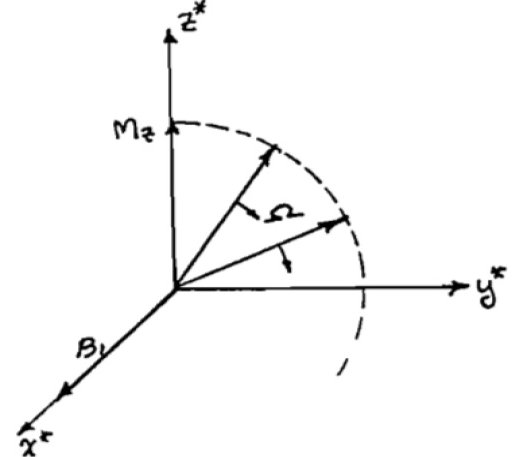
\includegraphics[width=\linewidth]{pic-de-manual/rotacion-de-coordenadas.jpg}
\label{fig:3}
\captionof{figure}{Rotating frame coordinates with M\textsubscript{z} 
precessing with angular velocity $\Omega$ \cite{ref:2}.}
\justify
The equation that will describe the motion of the spins in the Magnetic field 
is given by equation \ref{eqn:12}.
\begin{equation}
\frac{d\vec{M}}{dt} = \gamma\vec{M}\times B_{eff}^{*}
\label{eqn:12}
\cite{ref:2}
\end{equation}
The rotation of the M\textsubscript{z} field is equal to $\gamma B_1$.
\\
One of the most important concepts in PNMR that describes it as being pulsed is 
the use of strong RF pulses. They are exactly the ones that were introduced 
before with Hahn Spin Echo. There are three main different types of pulses that 
need to be introduced: 90\textsuperscript{o}, 180\textsuperscript{o} and
360\textsuperscript{o}. The pulses are known under this convention because 
they give the angle by which the angular momenta are displaced from their 
position prior to the pulse being applied. That is to say when the 90\textsuperscript{o} 
pulse is applied on the system the angular momenta may shift from the z-axis to 
the xy-plane. If the 180\textsuperscript{o} pulse is applied to the system the 
angular momenta shift from the z-axis to the -z-axis. All of these pulses have 
the exact same conditions except for the length of time by which they are 
applied. As such, the length of time that is needed by different materials may 
vary. The role that this has on the experiment is that as long as the spins are 
aligned with the z-axis measurements cannot be taken. Only when they are 
shifted to the xy-plane will they be able to give an FID signal and become 
measurable by the instruments. Due to the T\textsubscript{1} relaxation time 
the magnetization along the xy-plane will not hold for a very long amount of 
time and decay exponentially. This is represented on the figure below.
\center
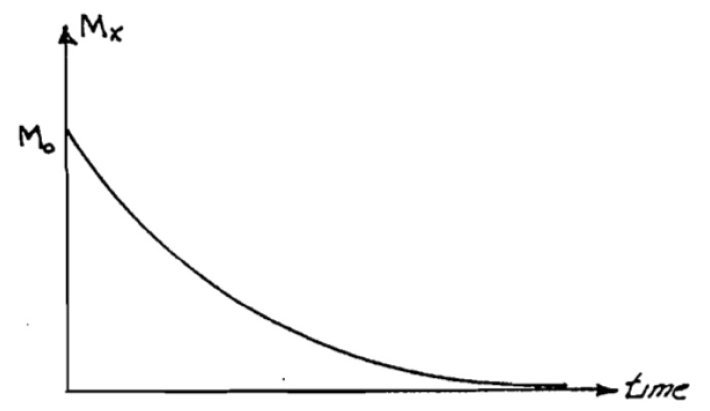
\includegraphics[width=\linewidth]{pic-de-manual/t2.jpg}
\captionof{figure}{Exponential decay of the Magnetization in the xy-plane as a 
function of time \cite{ref:2}.}
\label{fig:4}
\justify
So far, anything that has to do with the PNMR experiment has been largely 
dominated by the Spin-Lattice relaxation time. Now, let's see where the 
Spin-Spin relaxation time comes into play. Previpously it has been mentioned 
how the Hahn Spin Echo can appear without having a previous excitation from any 
RF pulse. Well this is actually due to the precessing spins on the xy-plane. 
The Hahn Spin Echo technique can be employed to measure the Spin-Spin 
relaxation times and the method makes use of a singular 90\textsuperscript{o} 
pulse followed by a after some time constant, $\tau$, a 180\textsuperscript{o} 
pulse. The importance of this sequence is that by pulsing with a 
90\textsuperscript{o} pulse the spins will be shifted from the thermal 
equilibrium axis to the 
xy-plane where after the time constant they will have precessed according to 
their Spin-Spin relaxation time. Now it is important to note that, the spins 
will split approximately half going one way and half the other way 
\cite{ref:1}. Also, the spins they do not all precess at the same rates. Some 
will be slower than others.
\\
By applying the second pulse, 180\textsuperscript{o}, the spins will flip on 
the xy-plane and continue to precess at their same rates and directions. Which 
means then, that the slower spins will be ahead of the faster precessing spins 
in the hope that they all come back and meet in the same place. As they precess 
the spins point in random directions and can be approximated to cancel each 
other out. It is only when they re-phase with one another that the Hahn Spin 
Echo signal can be viewed. A pictoral representation of this is shown on the 
figure below.
\center
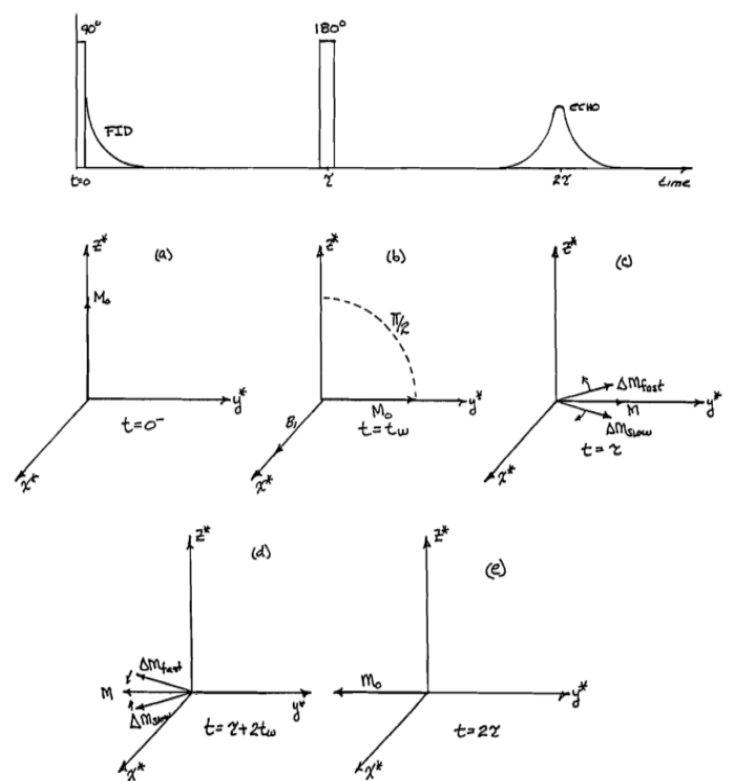
\includegraphics[width=\linewidth]{pic-de-manual/giro-de-momenta-angular.jpg}
\captionof{figure}{Top Figure: representation of the signal received from the 
instruments. (a) Initial state at thermal equilibrium. (b) A strong 
90\textsuperscript{o} RF pulse is applied on the system at resonance; the 
angular momenta shift to the xy-plane. (c) Angular momenta begin to precess on 
the xy-plane due to the Spin-Spin interactions. (d) A strong 
180\textsuperscript{o} RF pulse is applied and flips the angular momenta on the 
xy-plane. (e) Spins regain phase and give rise to the peak at time (2$\tau$) 
\cite{ref:2}.}
\label{fig:5}
\justify
However, the amount of time for which the spins are allowed to freely precess 
must be less than the Spin-Lattice relaxation time. Otherwise the spins will 
re-establish thermal equilibrium and applying a 180\textsuperscript{o} will not 
achieve any measurements. That is to say that the longer the $\tau$ value the 
lower the peak heigth of the Hahn Spin Echo. The equation relating the 
Spin-Spin relaxation time to the magnetization along the xy-plane is the 
following,
\begin{equation}
M_{x,y}(2\tau) = M_0 e^{-2\tau / T_2}
\cite{ref:1}
\label{eqn:13}
\end{equation}
Finally, one last mention that the above theoretical model is best applied on 
single nucleonic spins. When molecules are to be studied and even some larger 
atoms the magnetic field will be different due to the induced orbital motions 
of the electrons in the orbitals. 
Even the diamagnetic moment of some nearby atoms and molecules can greately 
affect the Larmour frequency of the nucleus being examined \cite{ref:1}.
\section{Experimental Set-Up}
As it was mentioned before, for this experiment TeachSpin's PS1-A spectrometer 
will be used. Figure 6 and 7 are a simplified block diagram of the set-up.
\center
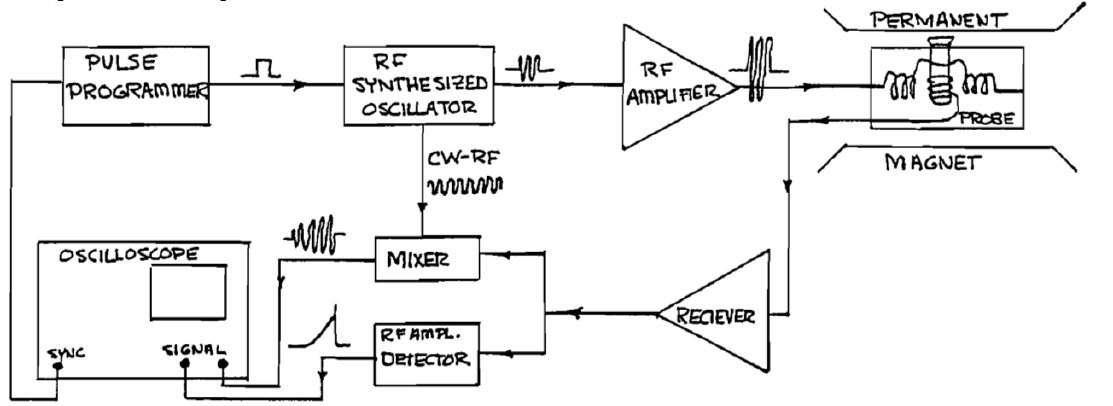
\includegraphics[width=\linewidth]{pic-de-manual/circuito.jpg}
\captionof{figure}{Simplified block diagram of the entire experimental set-up 
\cite{ref:2}.}
\label{fig:6}
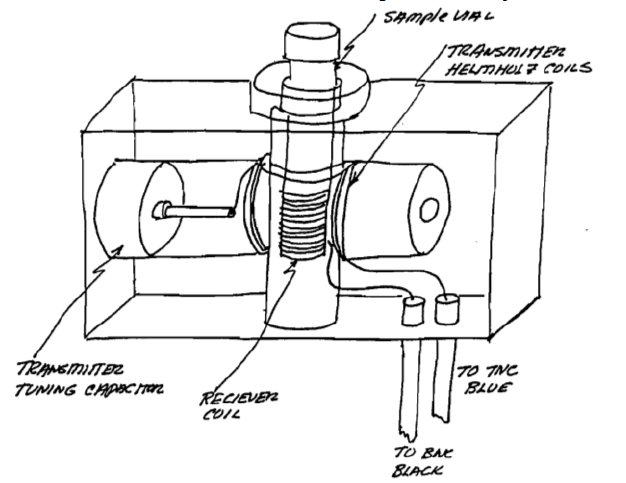
\includegraphics[width=\linewidth]{pic-de-manual/cajacentral.jpg}
\captionof{figure}{Close-up of the Magnet Diagram including the permanent 
magnet, receiver coils and the coils giving off the RF magnetic field \cite{ref:2}.}
\label{fig:7}
\justify
The coils giving off the B\textsubscript{1} are arranged in a helmholtz 
configuration to provide maximum field homogeneity to the sample. On Figure 
\ref{fig:6} the cycle starts from the oscilloscope, where the resonant 
frequency for the sample is set and sent to the pulse programmer. The pulse 
programmer takes care of transforming the input into the specific pulses. Whose 
width depends on the values that the knobs are set to, the knobs will be 
pointed out later. From there it moves through the rest of the circuit to the 
sample. going thorugh the wires and creating the RF fieldi \cite{ref:2}.
\\
Figures 8 and 9 show the controller unit that houses all the modules to perform 
the experiment and the magnet with the probe housing respectively.
\center
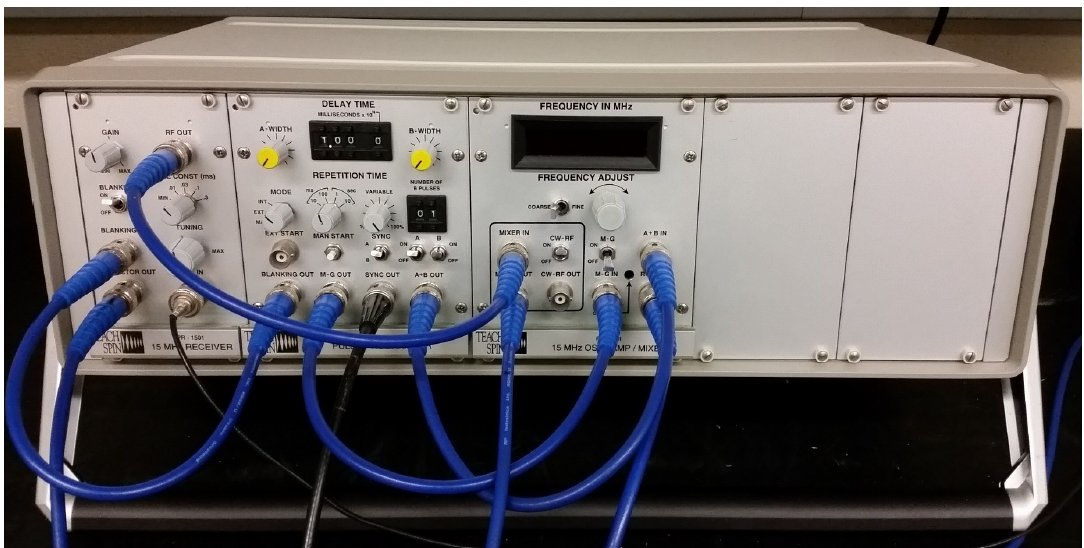
\includegraphics[width=\linewidth]{pic-de-manual/main-setup.jpg}
\captionof{figure}{Controller Unit the last two modules are empty for further expansions \cite{ref:2}}
\label{fig:8}
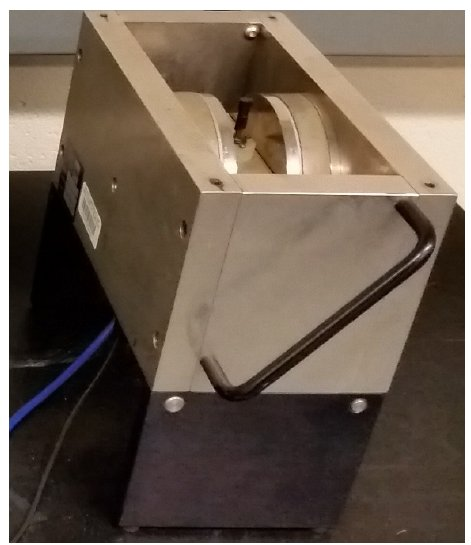
\includegraphics[width=\linewidth]{pic-de-manual/iman.jpg}
\captionof{figure}{Magnet Assembly housing permanent magnet and sample holder \cite{ref:2}.}
\label{fig:9}
\justify
The detector coil has two different outputs, one which goes to the mixer and 
one that goes to the detector out port on the controller unit. The mixer on the 
block diagram takes the frequency that is to be inputted into the coils and 
mixes it with the output of the detector. This will be important to remember 
for the actual experiment. The resonant frequency will be achieved when the 
beat output on the oscilator from the mixer output is nearly zero.
\\
The magnetic field due to the permanent magnet ha sbeen measured at the factory 
and all of the specs for the magnet will be included at the end of this 
section. The plastic cover that is on the magnet housing should be kept there when there is no need to immediately access the sample for any source of magnetic field could degrade the homogeneity of the field. Also, the magnets can be 
brittle so be careful with metal that is close to the magnet \cite{ref:2}.
\\
This magnet like many others is temperature dependent. However, since the 
temperature under which the magnetic field of the magnet was measured is 
unknown the following equation would not be of much use in calculating the 
resonant frequency.
\begin{equation}
\Delta H = 4gauss/^o C or 17kHz/^o C for protons
\end{equation}
There is a proportional relationship between the temperature of the magnet and 
the field strength. The temperature of the magnet should be kept as cool as 
possible to avoid too much drifting in the resonant frequency. It is very 
possible that it will need to be checked quite periodically in order to 
maintain the resonance condition \cite{ref:2}.
\\
The pulse programmer is shown on Figure \ref{fig:10} and it is a complete 
self-contained pulse generator. The controls are as follows: \\
\textbf{A-Width}: Width of A pulse between 1-30 $\mu$s. \\
\textbf{B-Width}: Width of B pulse between 1-30 $\mu$s. \\
\textbf{Delay Time}: Delay between the A and B pulses. Can be set to any number 
between 0.01 to 9.99e3 ms. \\
\textbf{Accuracy}: 1 pt in 10\textsuperscript{6} on all delay times. \\
\textbf{Mode}: Int (Internal): The pulse stream is repeated with a repetition time selected by the two controls on the right of the mode switch. \\
Ext (External): the pulse stream is repeated at the rising edge of an external TTL pulse. \\
Man (Manual): the pulse stream is repeated every time the manual start button is pushed. this allows the experimenter to choose arbitrarily long repetition times for the experiment. \\
\textbf{Repetition Time}: Sets the interval in between each measurement taken. 
The variable node next to it sets what percentage of it will be the value. \\
\textbf{Number of B pulses}: Number of B pulses from 0 to 99
\center
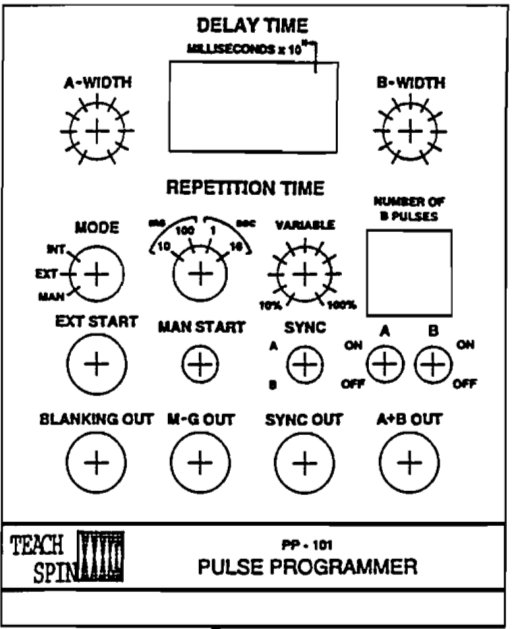
\includegraphics[width=\linewidth]{pic-de-manual/primerpanel.jpg}
\captionof{figure}{Pulse Programmer \cite{ref:2}.}
\label{fig:10}
\justify
\section{Results and Discussion}
(i) The Spectrometer \\
For this part of the experiment just had to hook up all of the cables according 
to the picture given, figure \ref{fig:13}.
\center
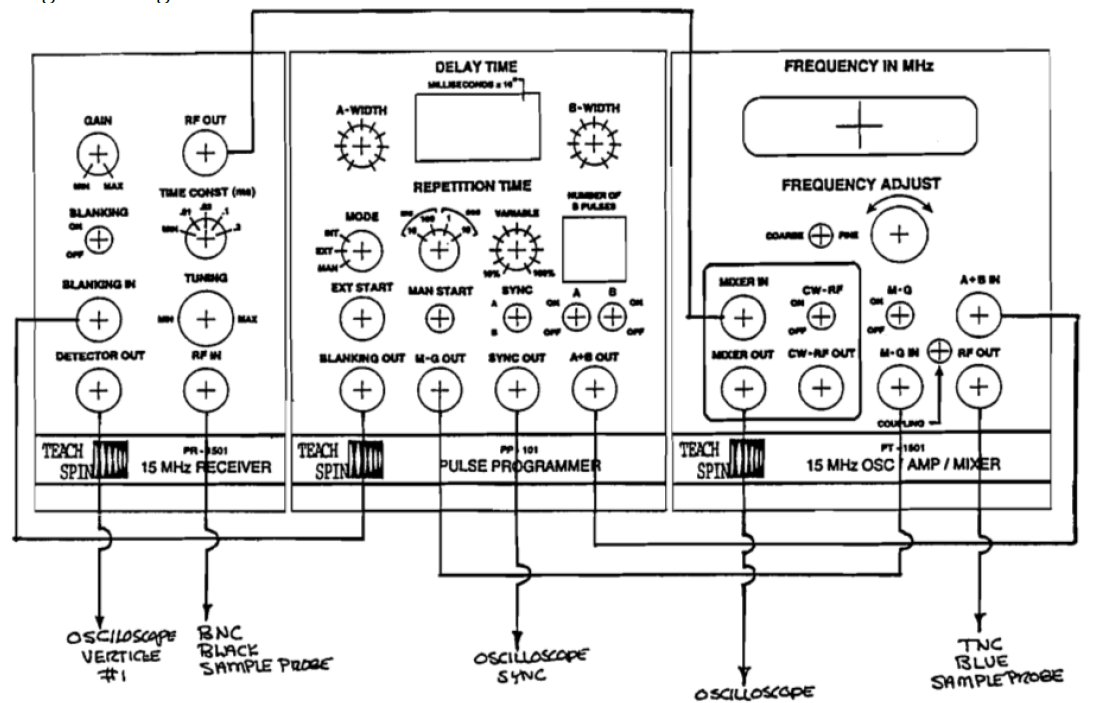
\includegraphics[width=\linewidth]{pic-de-manual/coneccionesdelpanel.jpg}
\captionof{figure}{Gives the schematics for which cables are supposed to go 
where.}
\label{fig:13}
\justify
(ii) Pulse Programmer \\
\\
For this section of the experiment just had to play with the pulse programmer 
and get aquaited with what all of the knobs and other buttons did. As expected 
when the scale settings for the time were changed the pulse got smaller and 
larger depending on which way we go with the scale. When the repetition 
variable scale was changed from 10\% to 100\% there was a change in the 
amplitude of the pulse.\\
\\
(iii) Pulse-Sequences \\
\\
As we changed the width of the pulses there did not seem to be much of a 
change. Looking back on it there may have been some errors made since nothing 
was seen to happen in terms of the spin echo. One possibility was that it was 
so far out of resonance that the spins never had enough of a precession to be 
able to create a strong enough signal to be able to see noticeable changes. 
Also, there was the problem of what to look at. \\
\\
(iv) Multiple Pulse Sequences \\
\\
In this part of the experiment we began to test what the Carr-Purcell and 
Meiboom-Gill method that would later be used would look like. As the number of 
pulses was increased all that seemed to increase was the number of pulses. 
Pulse width was the same for all, the B pulses but amplitude was the same. \\
\\
(v) The Receiver \\
\\
For this part of the experiment the resonant frequency had to be found 
experimentally. By using equation \ref{eqn:3} we could approximate the resonant 
frequency to approximately 14.903 MHz when we adjusted it experimentally we 
found that in the position that we were currently in it was more around 
15.422 MHz. I mention the current position since we would later go ahead and 
map out the magnet to find areas of uniformity and the frequency varied between 
the different areas in the magnet. \\
\\
(vi) Single Pulse NMR Experiment - FID \\
In this part of the experiment we were trying to get a FID signal from one 
single 90\textsuperscript{o} pulse at resonant conditions. Figure \ref{fig:14} 
shows our result for this part of the experiment.
\center
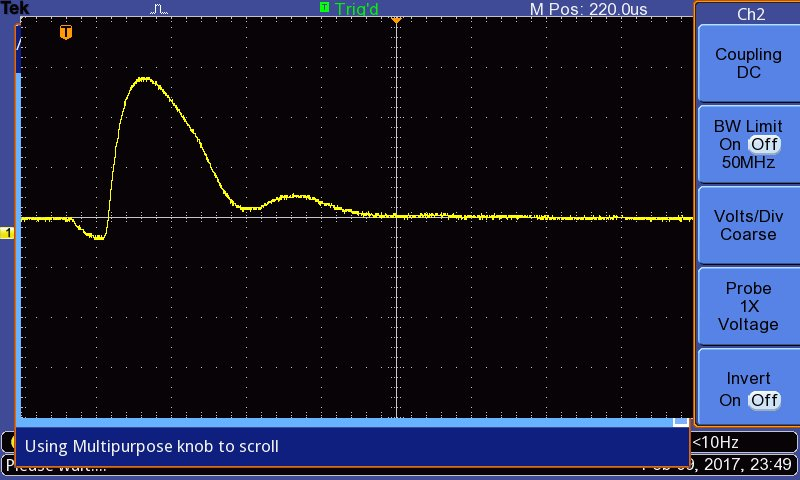
\includegraphics[width=\linewidth]{Early-Data/ALL0017/F0017TEK.jpg}
\captionof{figure}{Signal from the RF amplifier detector.}
\label{fig:14}
\justify
(vii) Magnetic Field Contours \\
\\
In this part of the experiment we tried to find the "sweet spot" of the magnet 
where the field would be most uniform. The importance of this is that we don't 
want a field which is not constant since then there is a posibility that the 
spins of the nucleons won't align themselves as well as they should if at all.
\\
For this part we chose to have a grid with a resolution of 0.5 units in the 
horizontal direction from -3 to +3 and a vertical resolution of 1.0 units from 
10 to 20 units. This in turn gave us a plot that looks like figure 
\ref{fig:15}. With the 
use of this figure it was determined that the "sweet spot" of the magnet would 
be at approximately 13 units in the vertical and -0.75 units in the horizontal. 
With an experimentally determined resonance value of 15.43 $\pm$ 0.02 MHz. We 
determined this error because from the RF coils the variance can be 17 kHz/
\textsuperscript{o}C. So it seems within reason to assume that the resonance 
would drift by more than that of 1\textsuperscript{o}C.
\center
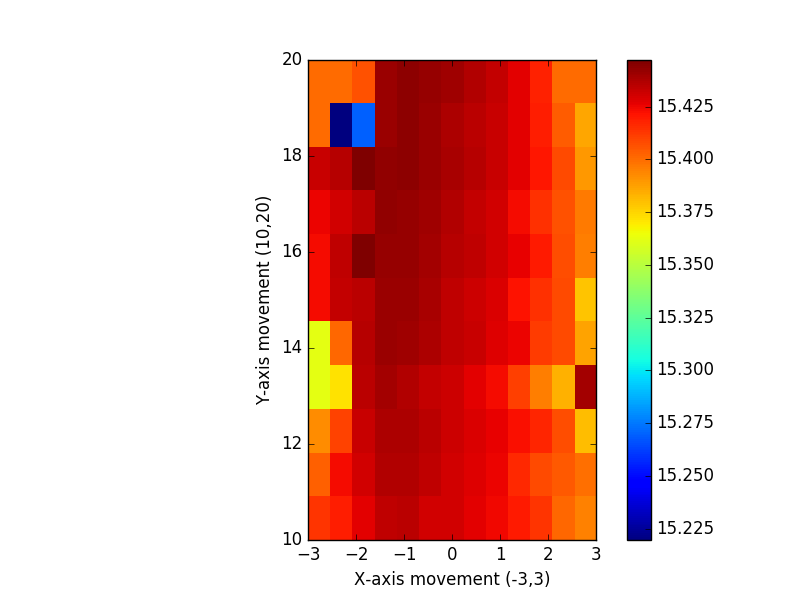
\includegraphics[width=\linewidth]{pic-for-report/magnet-colorplot.png}
\captionof{figure}{2D colorplot of the magnet homogeneity gotten using python.}
\label{fig:15}
\justify
(viii) Rotating coordinate systems \\
\\
It was determined that by using the channel 1 input of the oscilloscope the 
positions of the different pulse widths could be determined where the first 
90\textsuperscript{o} pulse was the first maximum from the minimum pulse width, 
180\textsuperscript{o} is the first minimum after the first maximum and so on.
\\
The reason for this is that at the 90\textsuperscript{o} the magnetization is 
pushed fully to the xy-plane and therefore has the greatest signal since we can 
only measure the signal in the xy-plane. At 180\textsuperscript{o} the 
magnetization is pointing along the -z-axis so it is almost the same as it 
being along the z-axis and there will not be any measuarable signal.
\\
It is not possible to create a total angular shift in the spins simply because 
it does not have the necessary energy to be able to cause the Zeeman transition into the excited that causes the spin to give off the signal as it relaxes.
\\
(ix) Spin Lattice relaxation time T\textsubscript{1} \\
\\
In this part of the experiment the Spin Lattice relaxation of mineral oil was 
found with two methods. The first was a sort of guess to approximate where to 
expect the zero for the data that we would take with the second method. For the 
second method screenshots of the oscilloscope were taken to collect the data of 
the spin magnetization when undergoing a 180\textsuperscript{o} - $\tau$ - 
90\textsuperscript{o} pulse sequence. Where $\tau$ is the delay time in 
milliseconds.
\\
With the first method we approximated the value to 38 $\pm$ 2 ms. The error was 
chosen as such due to the fact that within those two milliseconds there was 
very little noticeable change in the height of the peak. So, it became hard to 
determine the actual time.
\\
When using the data we got a value 37.7 $\pm$ 0.9 ms with an exponential fit 
using the curve\_fit tool in Python to fit to the fit equation 
$y = -Ae^{-kx} + B$. Where, x and y where the data points and all the rest were 
fit parameters. When we used the other method discussed in the theory section 
we got a value that when used in the actual experiment did not match up. The 
exponantial fit of the data is shown of figure \ref{fig:16}.
\center
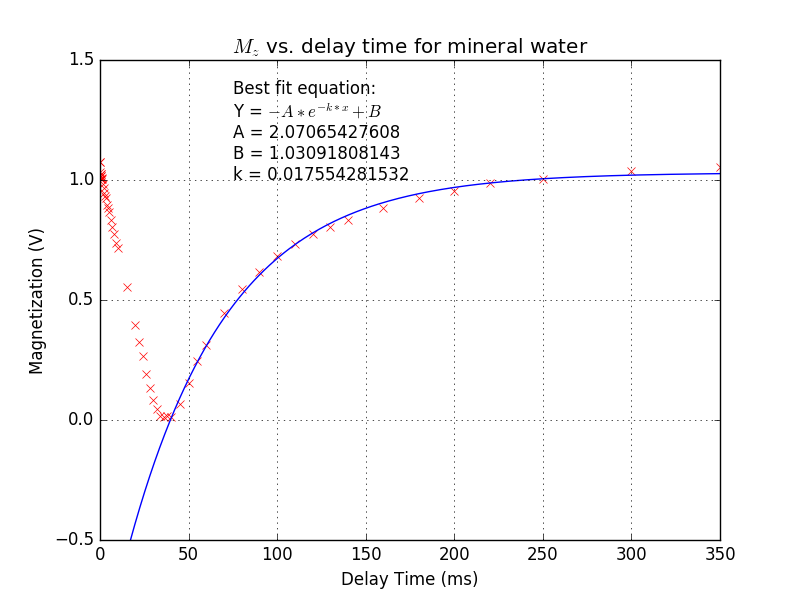
\includegraphics[width=\linewidth]{pic-for-report/mineral-water-T1.png}
\captionof{figure}{Exponential fit of data gotten to calculate the spin-lattice 
relaxation time of mineral oil.}
\label{fig:16}
\justify
(x) Spin-Spin relaxation time \\
\\
In this part of the experiment we used three different methods to find the 
Spin-Spin relaxation time of mineral oil: individual echo measurement, 
Carr-Purcell method and Meiboom-Gill method. For which we got values of 58.2 $\pm$ 
0.4 ms, 27.1 $\pm$ 0.9 and 54.8 $\pm$ 0.4 ms respectively. From the results it 
is clear that the other two methods completely outdid the Carr-Purcell method. 
The weakness in the Carr-Purcell method is that is the 180\textsuperscript{o} 
pulses are only a few degrees off it can really add up significantly as more 
and more pulses are observed dephasing the spins ever so slightly until they 
all point in random directions and the signals cancel themselves out.
\\
The plots of the exponential fits use the fit equation $y = -Ae^{-kx}$. Where, 
x and y are the data and A and k are the fit parameters.
\center
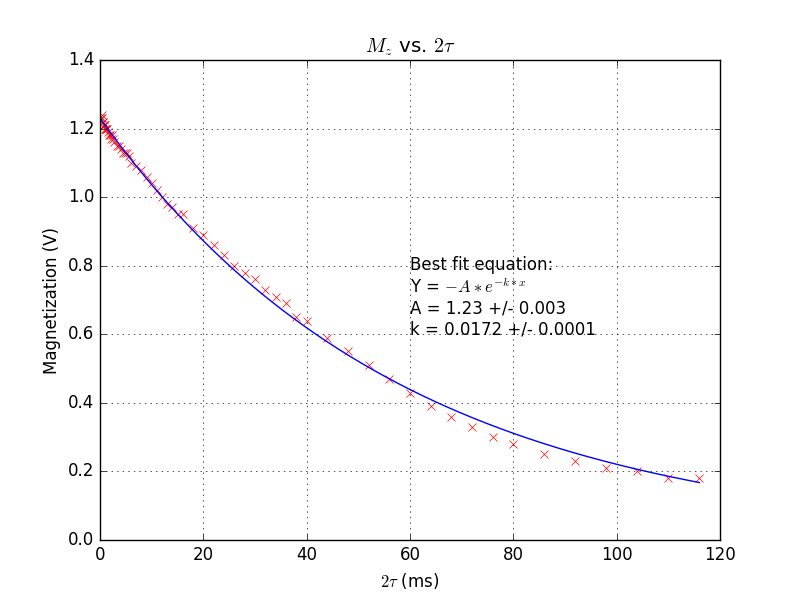
\includegraphics[width=\linewidth]{pic-for-report/mineral-water-T2.png}
\captionof{figure}{Mineral oil T2 with individual spin echo measurements.}
\label{fig:17}
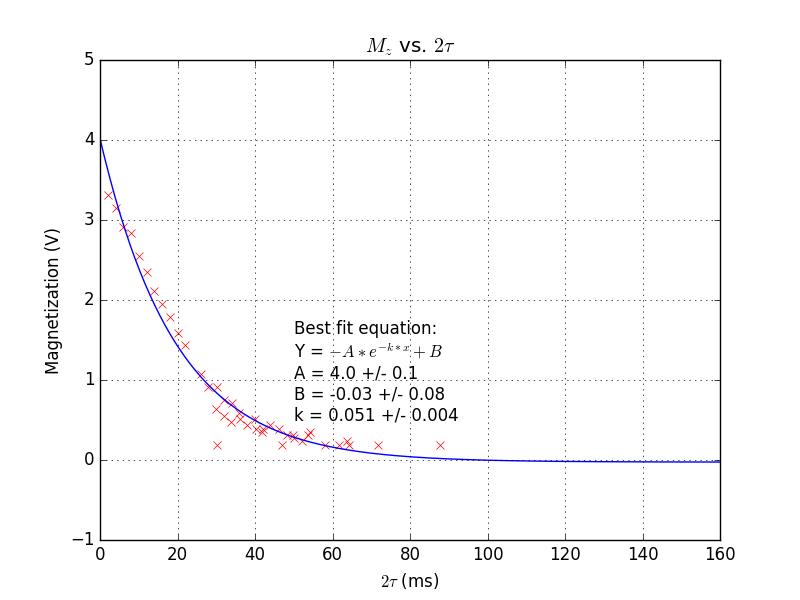
\includegraphics[width=\linewidth]{pic-for-report/mineral-water-T2-CP.png}
\captionof{figure}{Mineral oil T2 with Carr-Purcell method.}
\label{fig:18}
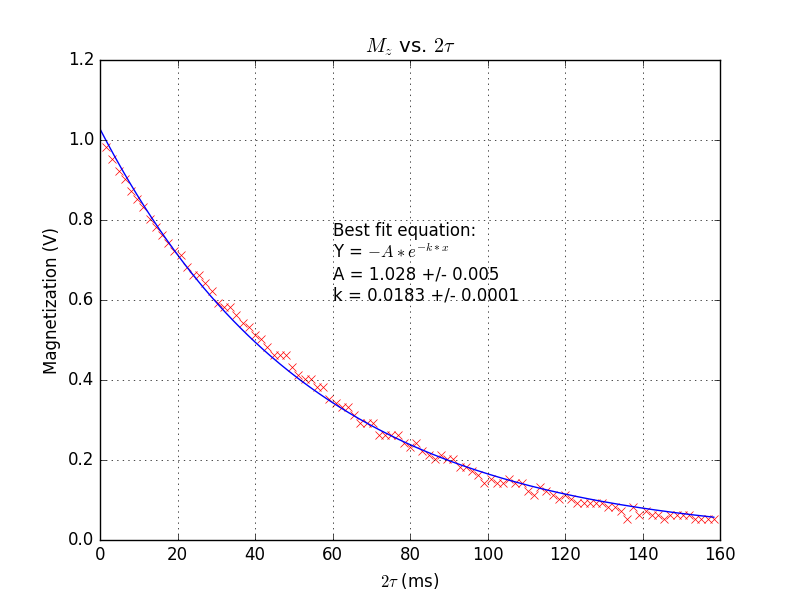
\includegraphics[width=\linewidth]{pic-for-report/mineral-water-T2-MG.png}
\captionof{figure}{Mineral oil T2 with Meiboom-Gill method.}
\label{fig:19}
\justify
(xi) CuSO\textsubscript{4} solutions \\
\\
In this part of the experiment we measured the Spin-Lattice and Spin-Spin 
relaxation times for 5 different solutions of Copper(II) Sulfate: 0.005M, 
0.010, 0.050M, 0.100M, 0.200M, 0.500M and 1.000M. The values for the relaxation 
times are shown in the following table.
\begin{tabular}{|c|c|c|c|c|}
\hline
 (M) & $T_1$ & $T_2$ & $1/T_1$ & $1/T_2$ \\ \hline
0.005 & 99 $\pm$ 8 & 98 $\pm$ 3 & 0.0101 & 0.0102 \\ \hline
0.010 & 61 $\pm$ 2 & 79 $\pm$ 1 & 0.0164 & 0.0127 \\ \hline
0.050 & 13.6 $\pm$ 0.2 & 17.3 $\pm$ 0.6 & 0.0735 & 0.0578 \\ \hline
0.100 & 6.5 $\pm$ 0.1 & 9.6 $\pm$ 0.3 & 0.1538 & 0.1042 \\ \hline
0.200 & 3.26 $\pm$ 0.06 & 4.5 $\pm$ 0.1 & 0.3067 & 0.2222 \\ \hline
0.500 & 1.25 $\pm$ 0.03 & 1.74 $\pm$ 0.05 & 0.8000 & 0.5747 \\ \hline
1.000 & 0.69 $\pm$ 0.01 & 0.93 $\pm$ 0.02 & 1.4493 & 1.0753 \\ \hline
\end{tabular}
The exponential fit functions are identical to those of the mineral oil. \\
There was a direct relationship between the molarity and the 1/$T_1$ and 1/$T_2$
 values. This makes sense because there are more copper spins present that will be able to be magnetized into the Zeeman splitting levels.
\center
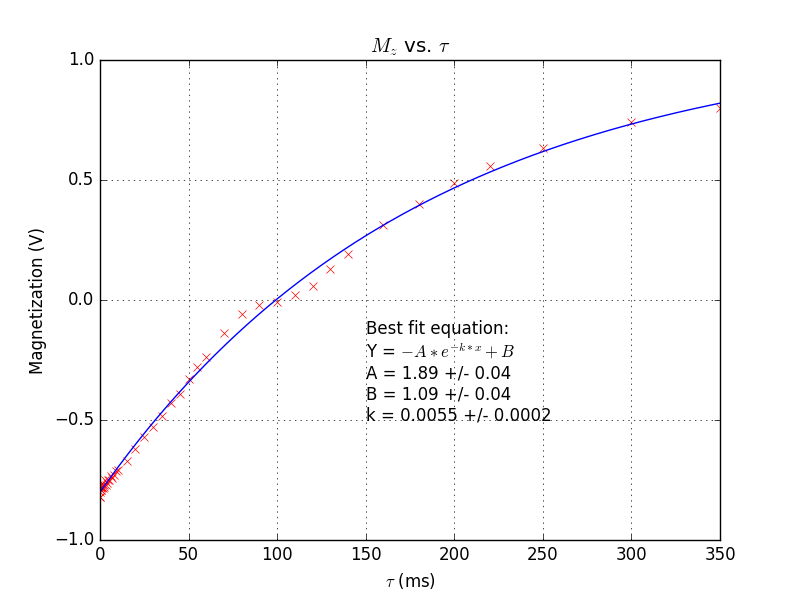
\includegraphics[width=\linewidth]{pic-for-report/a0005M-CuSO4-T1.png}
\captionof{figure}{Spin-Lattice relaxation of 0.005M Copper(II) Sulfate.}
\label{fig:20}
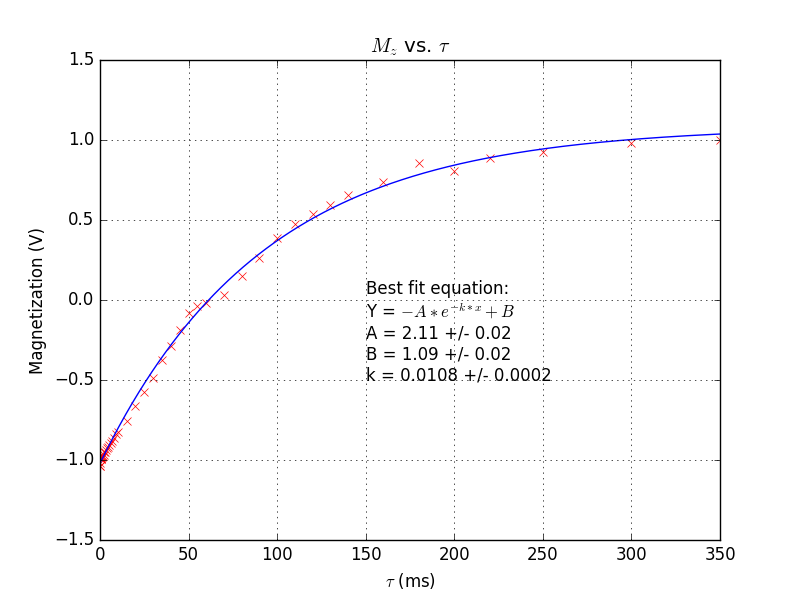
\includegraphics[width=\linewidth]{pic-for-report/a0010M-CuSO4-T1.png}
\captionof{figure}{Spin-Lattice relaxation of 0.010M Copper(II) Sulfate.}
\label{fig:21}
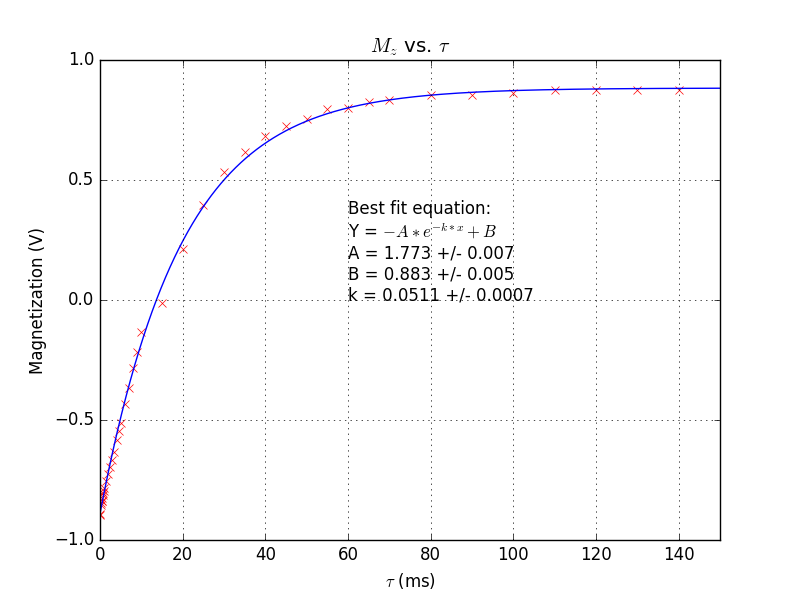
\includegraphics[width=\linewidth]{pic-for-report/a0050M-CuSO4-T1-inset.png}
\captionof{figure}{Spin-Lattice relaxation of 0.050M Copper(II) Sulfate.}
\label{fig:22}
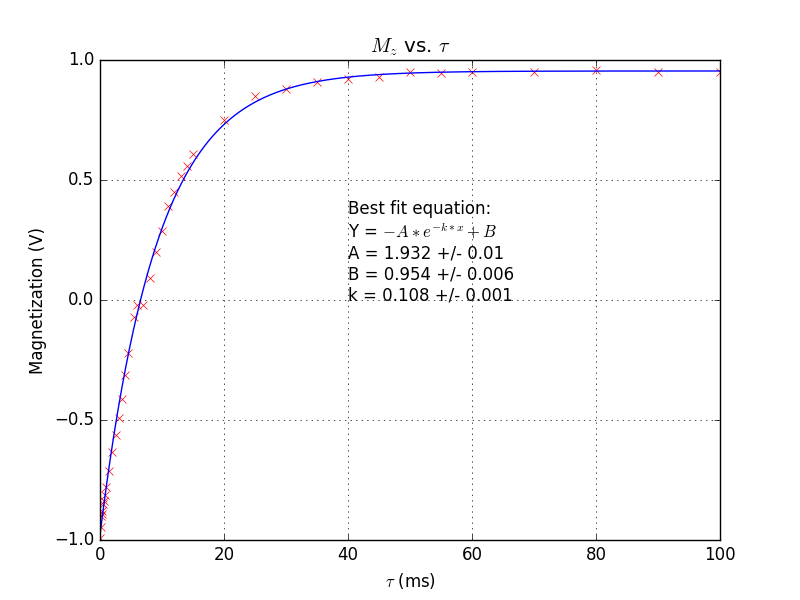
\includegraphics[width=\linewidth]{pic-for-report/a0100M-CuSO4-T1-inset.png}
\captionof{figure}{Spin-Lattice relaxation of 0.100M Copper(II) Sulfate.}
\label{fig:23}
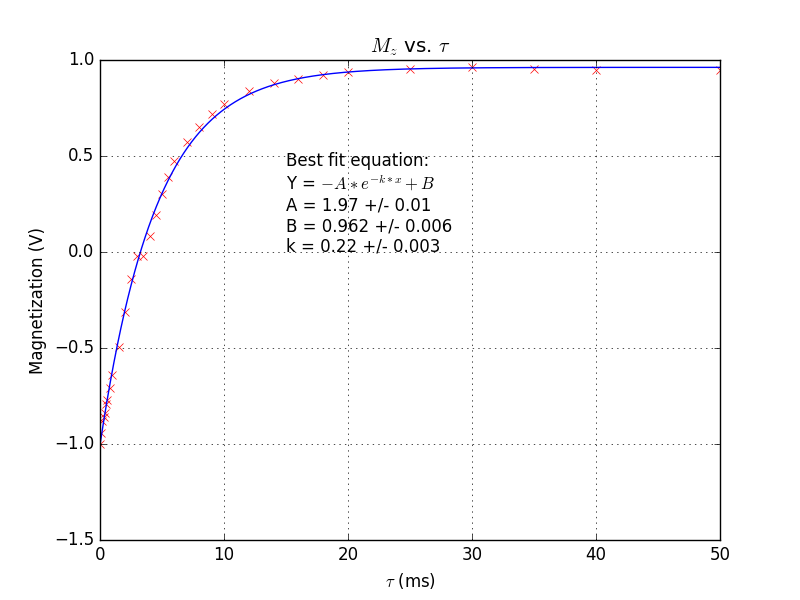
\includegraphics[width=\linewidth]{pic-for-report/a0200M-CuSO4-T1-inset.png}
\captionof{figure}{Spin-Lattice relaxation of 0.200M Copper(II) Sulfate.}
\label{fig:24}
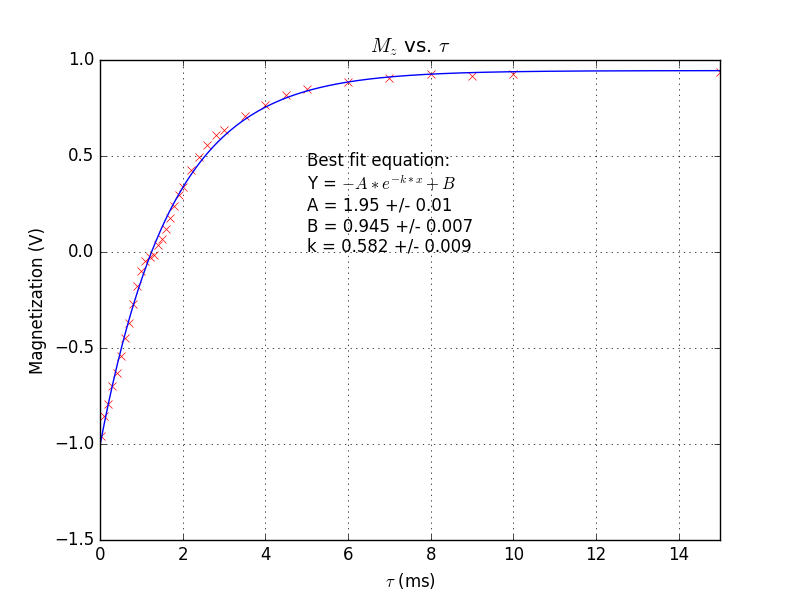
\includegraphics[width=\linewidth]{pic-for-report/a0500M-CuSO4-T1-inset.png}
\captionof{figure}{Spin-Lattice relaxation of 0.500M Copper(II) Sulfate.}
\label{fig:25}
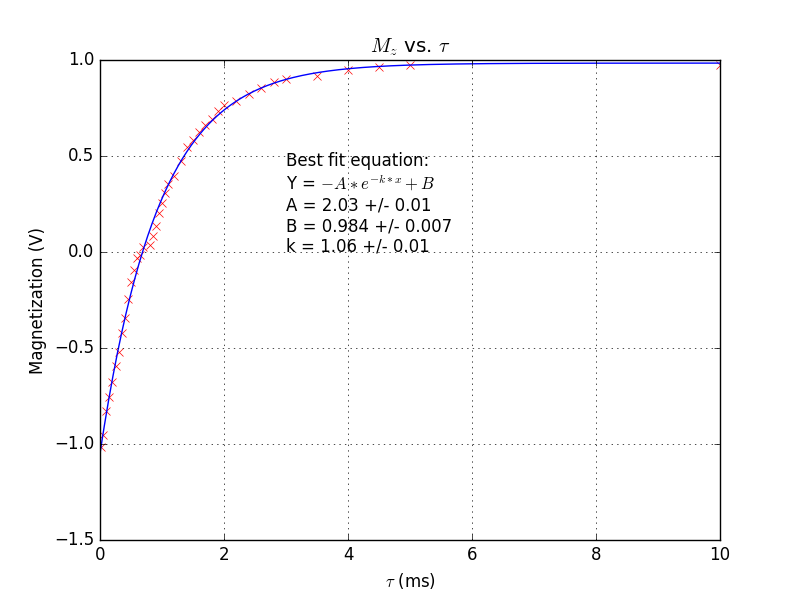
\includegraphics[width=\linewidth]{pic-for-report/a1000M-CuSO4-T1-inset.png}
\captionof{figure}{Spin-Lattice relaxation of 1.000M Copper(II) Sulfate.}
\label{fig:26}
\justify
For Spin-Spin Relaxation.
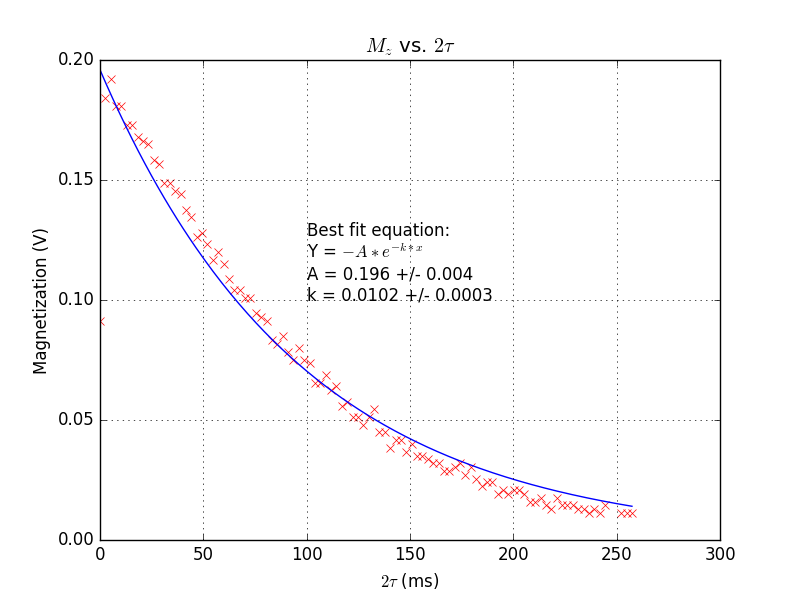
\includegraphics[width=\linewidth]{pic-for-report/a0005M-CuSO4-T2-MG.png}
\captionof{figure}{Spin-Spin relaxation of 0.005M Copper(II) Sulfate.}
\label{fig:27}
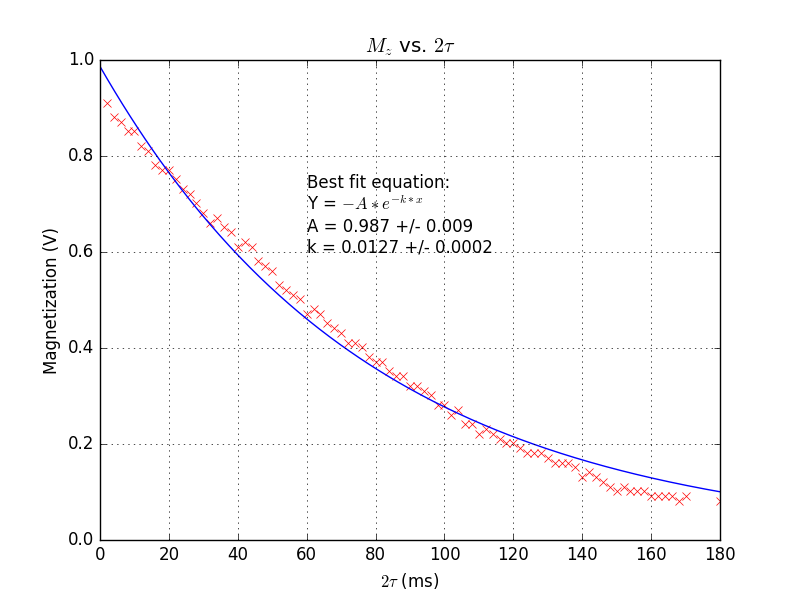
\includegraphics[width=\linewidth]{pic-for-report/a0010M-CuSO4-T2-MG.png}
\captionof{figure}{Spin-Spin relaxation of 0.010M Copper(II) Sulfate.}
\label{fig:28}
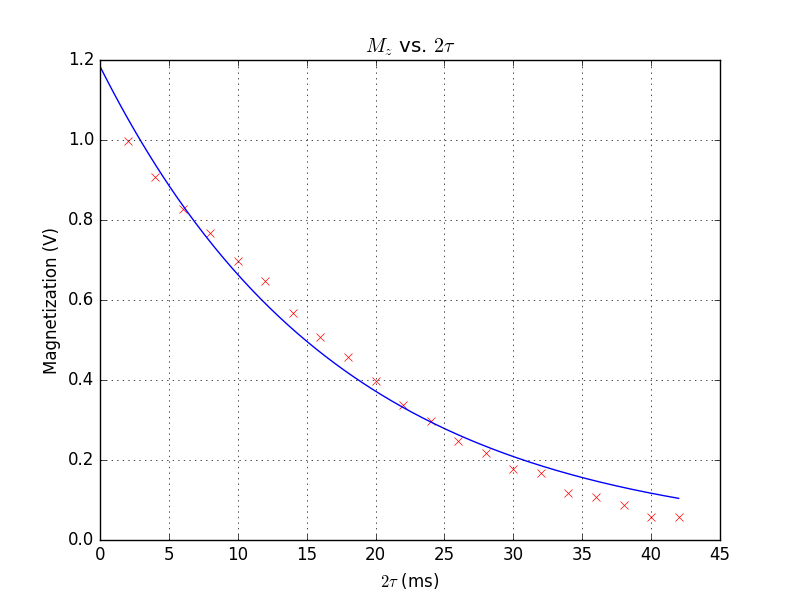
\includegraphics[width=\linewidth]{pic-for-report/a0050M-CuSO4-T2-MG.png}
\captionof{figure}{Spin-Spin relaxation of 0.050M Copper(II) Sulfate.}
\label{fig:29}
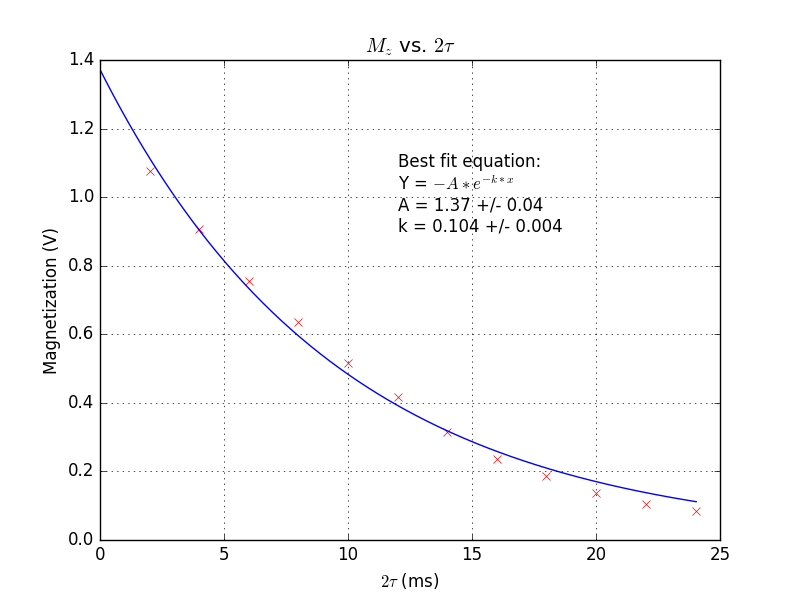
\includegraphics[width=\linewidth]{pic-for-report/a0100M-CuSO4-T2-MG.png}
\captionof{figure}{Spin-Spin relaxation of 0.100M Copper(II) Sulfate.}
\label{fig:30}
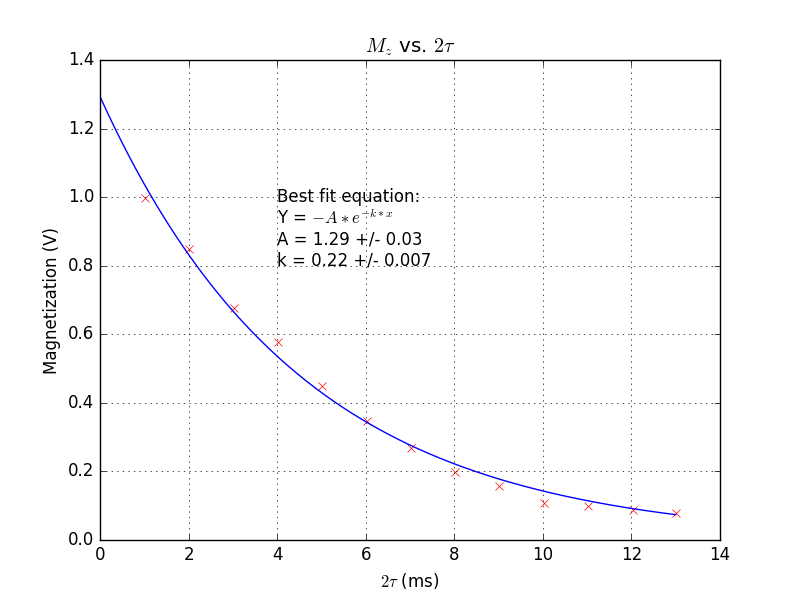
\includegraphics[width=\linewidth]{pic-for-report/a0200M-CuSO4-T2-MG.png}
\captionof{figure}{Spin-Spin relaxation of 0.200M Copper(II) Sulfate.}
\label{fig:31}
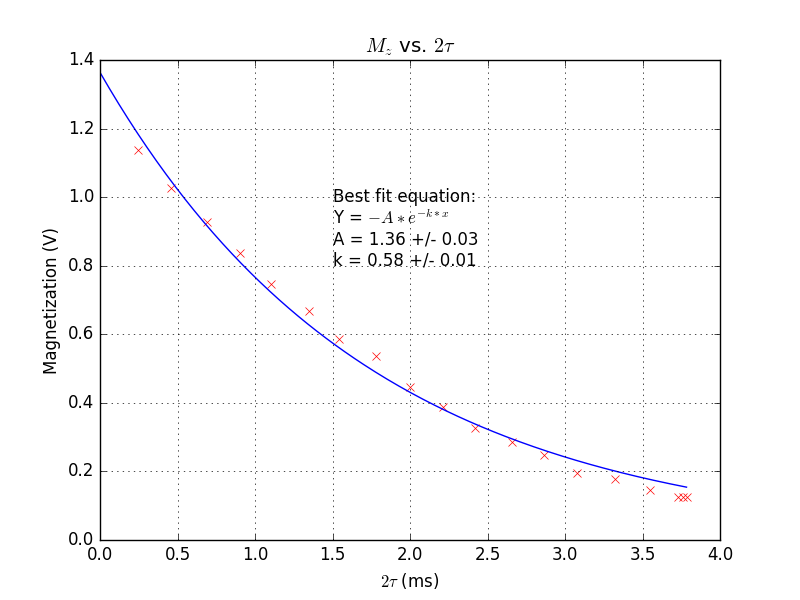
\includegraphics[width=\linewidth]{pic-for-report/a0500M-CuSO4-T2-MG.png}
\captionof{figure}{Spin-Spin relaxation of 0.500M Copper(II) Sulfate.}
\label{fig:32}
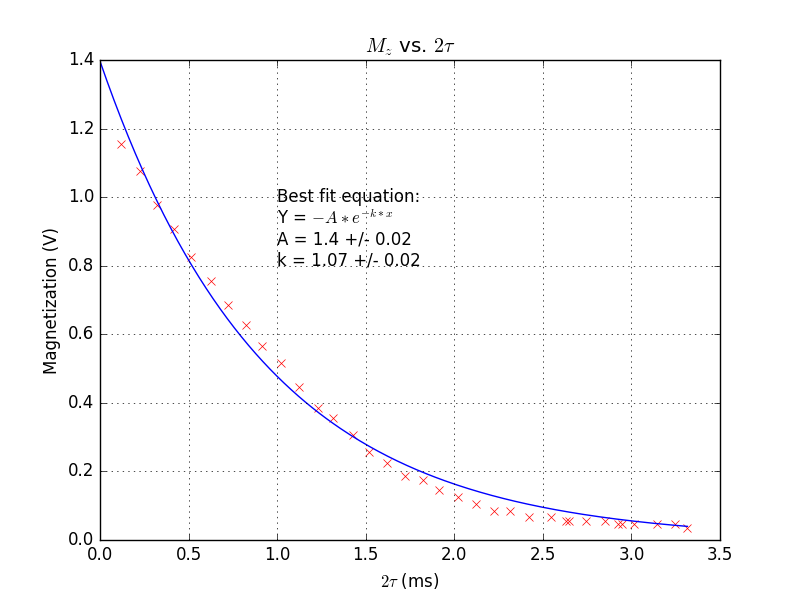
\includegraphics[width=\linewidth]{pic-for-report/a1000M-CuSO4-T2-MG.png}
\captionof{figure}{Spin-Spin relaxation of 1.000M Copper(II) Sulfate.}
\label{fig:33}
\justify
The Molar Concentration plots are the following.
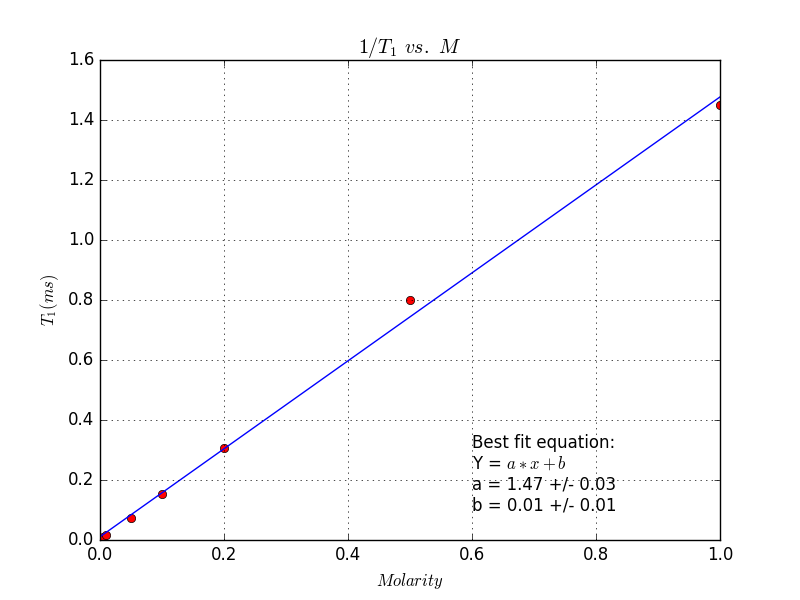
\includegraphics[width=\linewidth]{pic-for-report/t1-molar.png}
\captionof{figure}{Spin-Latice relaxation time vs. MolariltyCopper(II) Sulfate.}
\label{fig:34}
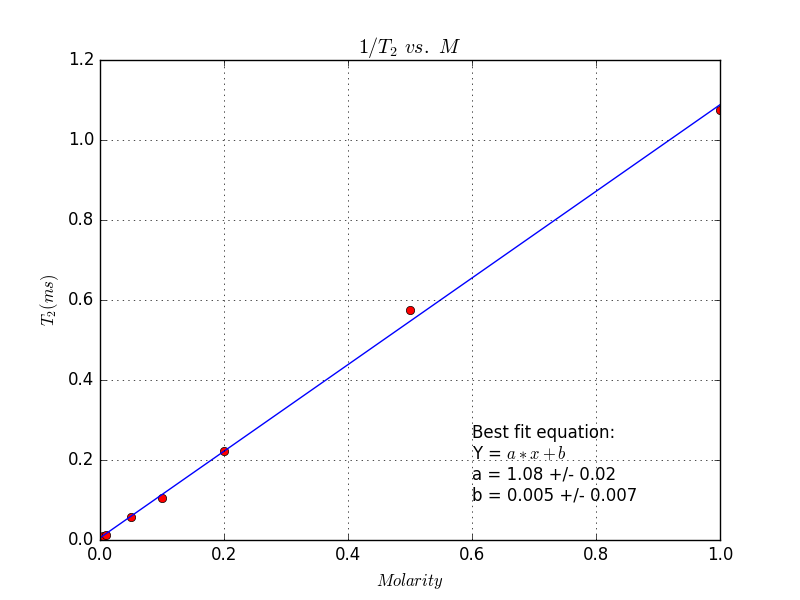
\includegraphics[width=\linewidth]{pic-for-report/t2-molar.png}
\captionof{figure}{Spin-Spin relaxation time vs. Molarity Copper(II) Sulfate.}
\label{fig:35}
\justify
(xii) Natural Products \\
\\
We chose Isoproponyl-2 alcohol as our natural product and got the values of 
570 $\pm$ 30 ms for the Spin-Lattice Relaxation time and 174 $\pm$ 3 ms for the Spin-Spin relaxation time.
\center
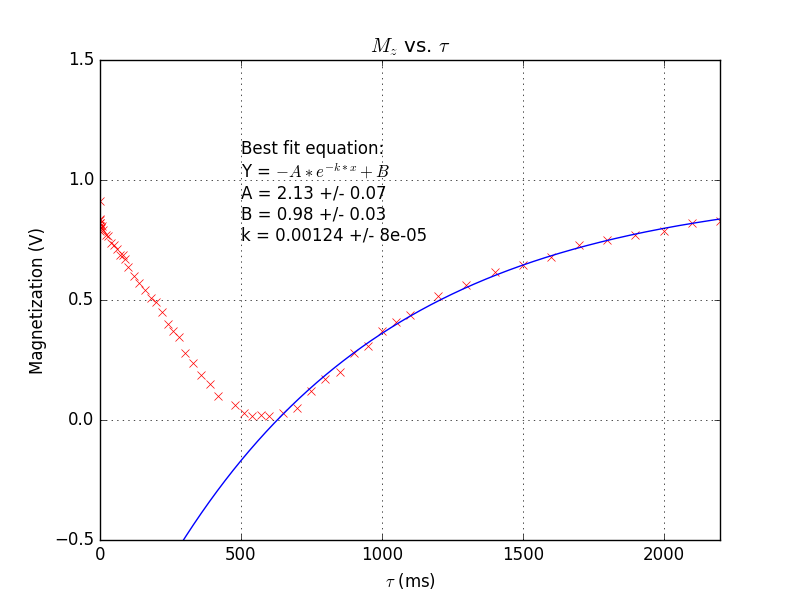
\includegraphics[width=\linewidth]{pic-for-report/isoproponyl-2-T1.png}
\captionof{figure}{Spin-Lattice relaxation of Isoproponyl-2 Alcohol.}
\label{fig:36}
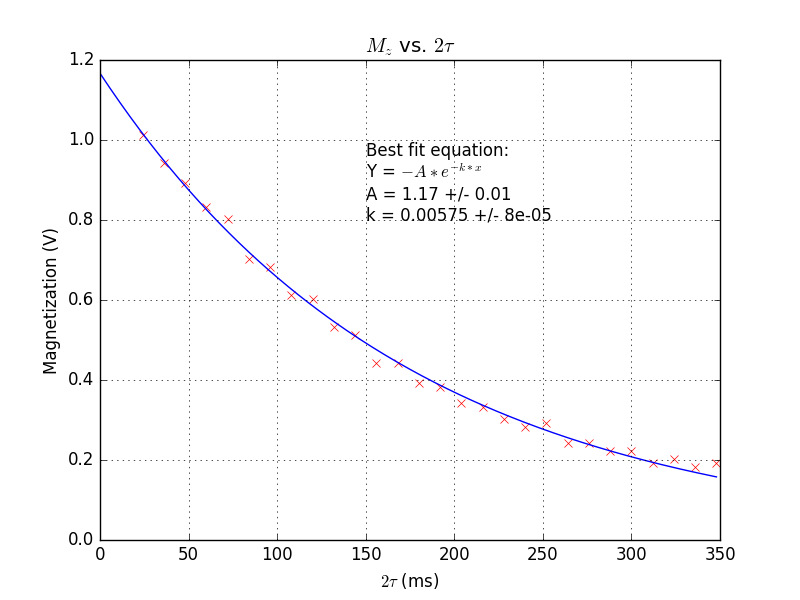
\includegraphics[width=\linewidth]{pic-for-report/isoproponyl-2-T2-MG.png}
\captionof{figure}{Spin-Lattice relaxation of Isoproponyl-2 Alcohol.}
\label{fig:37}
\justify
One of the possible reasons why our results for the alcohol are not as expected could be since it is an organic molecule it does have some extra factors that need to accounted for like those discussed at the end of the theory section.
\section{Conclusion}
PNMR is an extremely useful tool that has been used and developed over the past decades. Recently there have been many advances into the nano-scale NMR at non-cryogenic temperatures through the use Nitrogen-Vacant Diamond centers which have been able to achieve resolutions equal to or better than those of methods that use cryogenic temperatures.
\begin{thebibliography}{9}
\bibitem{ref:1}
Paudler, W. W. (1987) \emph{Nuclear Magnetic Resonance General 
Concepts and Applications}. John Wiley \& Sons Inc.
\bibitem{ref:2}
PHY 408 Lab manual. \emph{Pulsed NMR}
\bibitem{ref:3}
Ratner, M. A.; Schatz,G. C. (1993) \emph{Quantum Mechanics in Chemistry}. 
Englewood Cliffs, New Jersey : Prentice-Hall Inc.
\end{thebibliography}
\end{multicols}
}
\end{document}
